\chapter{What Is ``East Asia''? Geography and the Idea of a Region}

\section{Course framing}

The course asks two questions over and over: \emph{what do China, Japan and Korea share},
and \emph{why did they turn out so differently}? The professor's answer for the first half
of the term is a common ``cultural toolkit'' that spread outward from China (the writing
system, Confucian political ethics, Mahayana Buddhism, a model of bureaucratic
government). The second half is about how each society adapted that toolkit, and then how
each reacted to the arrival of Western powers in the nineteenth century.

\begin{important}[Three themes to track all term]
\begin{enumerate}
  \item \textbf{Shared heritage}: Chinese characters, Confucianism, Buddhism, the
        imperial/tributary model of the world.
  \item \textbf{Local adaptation}: each society kept what was useful and reshaped it
        (kana, hangul, samurai rule, Korean neo-Confucian orthodoxy).
  \item \textbf{Divergent modernities}: after 1840 the three countries took very different
        roads (semi-colonial China, imperial Japan, colonized Korea), which explains much
        of today's politics.
\end{enumerate}
\end{important}

\section{Where is ``East Asia''?}

``East Asia'' is a \emph{constructed} region. There is no natural line that separates it
from Southeast, Central or North Asia. In this course it means the \emph{cultural sphere}
that used Chinese characters and was shaped by Confucian and Buddhist institutions:
China, Korea, Japan and (often) Vietnam. The course covers only the first three; Vietnam
is mentioned as a fourth member of the ``character sphere'' whenever it is useful.

\begin{definition}[Sinosphere / ``character cultural sphere'']
The \emph{Sinosphere} is the set of societies historically using Literary Chinese as a
written language of government and learning. In East Asian languages it is called the
``Chinese character cultural sphere'': \zht{漢字文化圈} (Hànzì wénhuà quān),
\ja{漢字文化圏} (kanji bunka-ken), \ko{한자 문화권} (hanja munhwagwon).
\end{definition}

\begin{remark}
The term ``Far East'' (still used in older books) is Eurocentric: far from \emph{where}?
The professor asked us to avoid it except when quoting sources.
\end{remark}

\subsection{Physical geography as a diagram}

No need to memorise maps in detail, but know the rough layout and why it
mattered.

\begin{center}
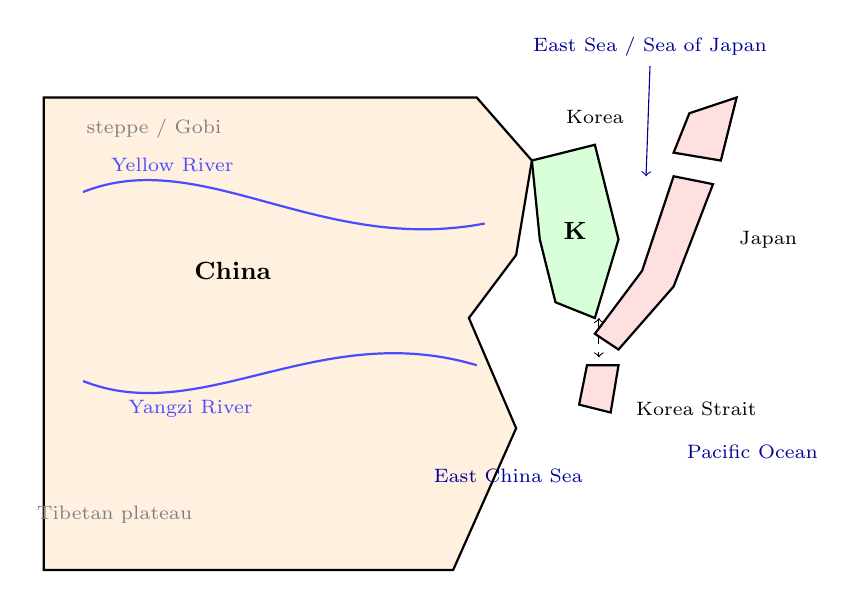
\begin{tikzpicture}[x=1cm,y=1cm, every node/.style={font=\small}]
  % China landmass
  \draw[thick, fill=orange!12] (-5,-3) -- (-5,3) -- (0.5,3) -- (1.2,2.2) -- (1.0,1.0)
      -- (0.4,0.2) -- (1.0,-1.2) -- (0.2,-3) -- cycle;
  \node at (-2.6,0.8) {\textbf{China}};
  % rivers
  \draw[blue!70, thick] (-4.5,1.8) .. controls (-3,2.4) and (-1.5,1.0) .. (0.6,1.4)
      node[pos=0.25, above, font=\scriptsize] {Yellow River};
  \draw[blue!70, thick] (-4.5,-0.6) .. controls (-3,-1.2) and (-1.5,0.2) .. (0.5,-0.4)
      node[pos=0.3, below, font=\scriptsize] {Yangzi River};
  % Tibet plateau / deserts
  \node[font=\scriptsize, gray] at (-4.1,-2.3) {Tibetan plateau};
  \node[font=\scriptsize, gray] at (-3.6,2.6) {steppe / Gobi};
  % Korea peninsula
  \draw[thick, fill=green!15] (1.2,2.2) -- (2.0,2.4) -- (2.3,1.2) -- (2.0,0.2) -- (1.5,0.4)
      -- (1.3,1.2) -- cycle;
  \node at (1.75,1.3) {\textbf{K}};
  \node[font=\scriptsize] at (2.0,2.75) {Korea};
  % Japan islands
  \draw[thick, fill=red!12] (3.2,2.8) -- (3.8,3.0) -- (3.6,2.2) -- (3.0,2.3) -- cycle;
  \draw[thick, fill=red!12] (3.0,2.0) -- (3.5,1.9) -- (3.0,0.6) -- (2.3,-0.2) -- (2.0,0.0)
      -- (2.6,0.8) -- cycle;
  \draw[thick, fill=red!12] (1.9,-0.4) -- (2.3,-0.4) -- (2.2,-1.0) -- (1.8,-0.9) -- cycle;
  \node[font=\scriptsize] at (4.2,1.2) {Japan};
  % seas
  \node[font=\scriptsize, blue!60!black] at (0.9,-1.8) {East China Sea};
  \node[font=\scriptsize, blue!60!black, anchor=south] (es) at (2.7,3.4) {East Sea / Sea of Japan};
  \draw[->, blue!60!black, thin] (es.south) -- (2.65,2.0);
  \draw[<->, dashed] (2.05,0.2) -- (2.05,-0.3);
  \node[font=\scriptsize, anchor=west] at (2.4,-0.95) {Korea Strait};
  \node[font=\scriptsize, blue!60!black] at (4.0,-1.5) {Pacific Ocean};
\end{tikzpicture}
\end{center}

\begin{itemize}
  \item \textbf{China} is a continental state. Its core is the North China Plain (Yellow
        River) and the Yangzi valley. To the north and west are steppe, desert and the
        Tibetan plateau: these are the zones of the nomadic peoples who repeatedly
        threatened, and twice conquered, the agrarian empire (Mongols, Manchus).
  \item \textbf{Korea} is a peninsula attached to the continent. It has always had to
        manage relations with whatever power controlled Manchuria and north China. Its
        mountains made unification slow (Three Kingdoms).
  \item \textbf{Japan} is an archipelago separated from Korea by about 200 km of sea. This
        distance let Japan \emph{choose} what to borrow and when to stop borrowing; it was
        never conquered by a continental power before 1945.
\end{itemize}

\begin{aside}
Mnemonic: ``\textbf{C}ontinent, \textbf{P}eninsula, \textbf{A}rchipelago''
explains a lot of the political history. China absorbs, Korea negotiates, Japan selects.
It is an oversimplification, but a useful one for essay outlines.
\end{aside}

\subsection{Naming the sea}

The body of water between Korea and Japan is ``Sea of Japan'' in most Western atlases
(\ja{日本海}, Nihonkai) but ``East Sea'' in Korea (\ko{동해}, Donghae). The dispute
shows that even geography is political in this region. Similar disputes: the islets
called Dokdo (\ko{독도}) by Korea and Takeshima (\ja{竹島}) by Japan; the
Diaoyu/Senkaku islands claimed by China and Japan.

\section{Names of the three countries}

\begin{center}
\begin{tabular}{llll}
\toprule
Country & Own name & Romanization & Literal meaning \\
\midrule
China & \zh{中国} & Zhōngguó & ``Central state(s)'' \\
Japan & \ja{日本} & Nihon / Nippon & ``Origin of the sun'' \\
South Korea & \ko{한국} (\zht{韓國}) & Hanguk & ``State of the Han (people)'' \\
North Korea & \ko{조선} (\zht{朝鮮}) & Chosŏn & ``Morning calm'' (traditional gloss) \\
\bottomrule
\end{tabular}
\end{center}

\begin{example}[Names as worldviews]
\zh{中国} places China at the centre of the world. \ja{日本} names Japan by its position
\emph{relative to China}: it is where the sun rises when seen from the continent. The
Japanese court adopted the name in the late 7th century in correspondence with the Tang
court. Both names presuppose a China-centred map of the world, which is the subject of the
tributary-system lecture.
\end{example}

\section{How the region has been studied}

\subsection{Orientalism}

The lecture introduced Edward Said's critique (\emph{Orientalism}, 1978): Western scholars
and writers created an image of ``the Orient'' as timeless, exotic, irrational and
passive, as the opposite of a modern, rational West. That image justified imperial
intervention.

\begin{important}[Avoid in essays]
\begin{itemize}
  \item Treating ``Asian culture'' as unchanging (``the Chinese have always\ldots'').
  \item Treating China, Japan and Korea as interchangeable.
  \item Explaining everything by ``Confucianism'' (the ``Confucian catch-all'').
\end{itemize}
\end{important}

\subsection{Area studies}

``East Asian Studies'' as a university field grew in North America after 1945, partly
funded for Cold War reasons (knowing the enemy and the ally). This history is one reason
the field has long emphasised language training and political history.

\section{Periodization: a first comparative timeline}

Every later lecture hangs on this chart. Dates are approximate and conventional.

\begin{center}
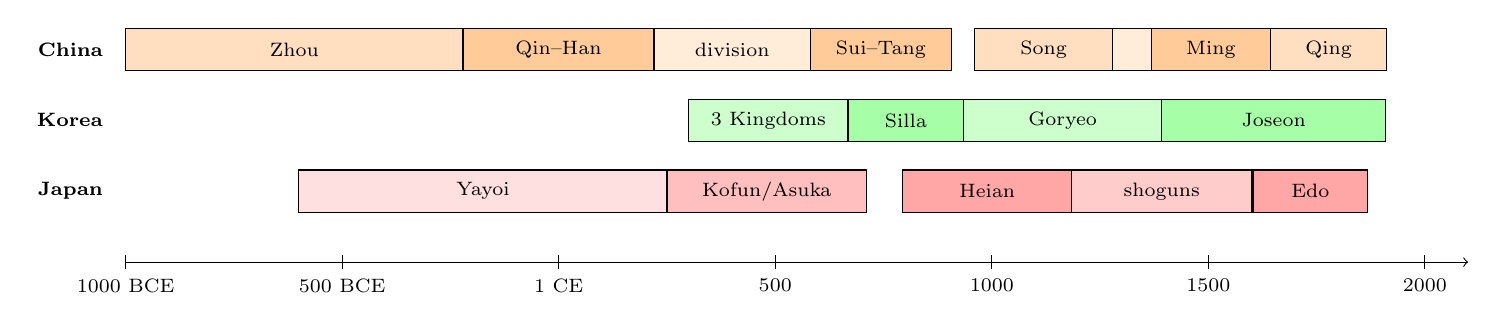
\begin{tikzpicture}[x=0.55cm, y=0.9cm, every node/.style={font=\scriptsize}]
  % axis from -1000 to 2000 => units of 100 years; x = (year+1000)/100 * 0.55
  \draw[->] (0,0) -- (31,0);
  \foreach \yr/\lab in {0/1000 BCE, 5/500 BCE, 10/1 CE, 15/500, 20/1000, 25/1500, 30/2000} {
    \draw (\yr,0.1) -- (\yr,-0.1) node[below] {\lab};
  }
  % China row
  \node[anchor=east] at (-0.3,3) {\textbf{China}};
  \draw[fill=orange!25] (0,2.7) rectangle (7.79,3.3) node[midway] {Zhou};
  \draw[fill=orange!40] (7.79,2.7) rectangle (12.2,3.3) node[midway] {Qin--Han};
  \draw[fill=orange!15] (12.2,2.7) rectangle (15.81,3.3) node[midway] {division};
  \draw[fill=orange!40] (15.81,2.7) rectangle (19.07,3.3) node[midway] {Sui--Tang};
  \draw[fill=orange!25] (19.6,2.7) rectangle (22.79,3.3) node[midway] {Song};
  \draw[fill=orange!15] (22.79,2.7) rectangle (23.68,3.3);
  \draw[fill=orange!40] (23.68,2.7) rectangle (26.44,3.3) node[midway] {Ming};
  \draw[fill=orange!25] (26.44,2.7) rectangle (29.12,3.3) node[midway] {Qing};
  % Korea row
  \node[anchor=east] at (-0.3,2) {\textbf{Korea}};
  \draw[fill=green!20] (13.0,1.7) rectangle (16.68,2.3) node[midway] {3 Kingdoms};
  \draw[fill=green!35] (16.68,1.7) rectangle (19.35,2.3) node[midway] {Silla};
  \draw[fill=green!20] (19.35,1.7) rectangle (23.92,2.3) node[midway] {Goryeo};
  \draw[fill=green!35] (23.92,1.7) rectangle (29.1,2.3) node[midway] {Joseon};
  % Japan row
  \node[anchor=east] at (-0.3,1) {\textbf{Japan}};
  \draw[fill=red!12] (4,0.7) rectangle (12.5,1.3) node[midway] {Yayoi};
  \draw[fill=red!25] (12.5,0.7) rectangle (17.1,1.3) node[midway] {Kofun/Asuka};
  \draw[fill=red!35] (17.94,0.7) rectangle (21.85,1.3) node[midway] {Heian};
  \draw[fill=red!20] (21.85,0.7) rectangle (26.0,1.3) node[midway] {shoguns};
  \draw[fill=red!35] (26.03,0.7) rectangle (28.68,1.3) node[midway] {Edo};
\end{tikzpicture}
\end{center}

\begin{remark}
Gaps in the Korea row before about 300 CE are not empty history: there were earlier
states (Gojoseon, the Han commanderies, Buyeo, the Samhan confederations). The chart only
shows periods we will use. The small unlabelled block in the China row is the Yuan
(Mongol) dynasty, 1271--1368.
\end{remark}

\section{Population and scale (for perspective)}

\begin{center}
\begin{tabular}{lrrl}
\toprule
 & Population (c.\ 2018) & Area (km$^2$) & Capital \\
\midrule
PRC & 1.39 billion & 9.6 million & Beijing \zh{北京} \\
Japan & 127 million & 378\,000 & Tokyo \ja{東京} \\
South Korea & 51 million & 100\,000 & Seoul \ko{서울} \\
North Korea & 25 million & 120\,000 & Pyongyang \ko{평양} \\
Taiwan (ROC) & 23 million & 36\,000 & Taipei \zht{臺北} \\
\bottomrule
\end{tabular}
\end{center}

China dwarfs its neighbours, which matters for everything from premodern diplomacy to
contemporary trade. The asymmetry is part of why Korea and Japan defined themselves
\emph{in relation to} China.

\section*{Summary}
\begin{itemize}
  \item ``East Asia'' is a constructed region, best defined culturally as the
        Chinese-character sphere (China, Korea, Japan, Vietnam).
  \item Geography (continent, peninsula, archipelago) shaped each society's relationship
        to the Chinese centre.
  \item Country names encode a China-centred worldview.
  \item Be wary of Orientalist generalizations and of explaining everything by
        ``Confucianism''.
  \item Learn the comparative timeline: it is the scaffolding for the whole course.
\end{itemize}
